\chapter{Introduction}
\label{ch:introduction}
This chapter provides the context for our thesis and outlines the problem we aim to address. Firstly, we highlight the necessity for XAI in making complex models more interpretable to users and introduce saliency maps as a potential solution. We then present the disagreement problem, which arises when different XAI methods provide conflicting explanations for a complex black box. Ultimately, we state the goal of our thesis to explore the extent of disagreement among saliency methods, an area that has yet to receive extensive research attention.

\section{Overview}
%Trong những năm gần đây, ta đã chứng kiến sự phổ biến và sức mạnh của các mô hình học sâu (Deep Learning models) trong nhiều loại ứng dụng khác nhau trong đời sống thực tiễn. Sức mạnh của các mô hình học sâu này được tăng cường theo từng ngày. Sự phát triển mạnh mẽ về tài nguyên tính toán cho phép các mô hình ngày càng trở nên lớn hơn và phức tạp hơn về mặt kích thước như là số lượng tham số và độ sâu. Ngoài ra, việc đầu tư mạnh mẽ vào nghiên cứu đã khuyến khích phát triển nên các kiến trúc đạt hiệu suất cao hơn nhưng cũng làm chúng trở nên phức tạp hơn với những người sử dụng.

In recent years, we have witnessed the rising popularity and effectiveness of deep learning models across diverse real-world applications. The power of these deep learning models has been amplified as the massive growth in computational resources allows models to become increasingly larger and more complex in dimensions, as evidence in the growing number of parameters and depth. Moreover, substantial investment in research has encouraged the development of more efficient architectures but has also made them more complex for users.

%Trong nhiều lĩnh vực thực tế, các hệ thống trí tuệ nhân tạo có thể được sử dụng để đưa ra các quyết định quan trọng có thể ảnh hưởng đến tính mạng của con người như y tế, an ninh hay tự động hóa. Chính vì thế, khi ứng dụng trí tuệ nhân tạo để giải quyết vấn đề, việc hiểu rõ lý do và quy trình mà một mô hình học máy sử dụng để đưa ra quyết định trở nên vô cùng quan trọng.

In some high-stake domains, artificial intelligence systems play a pivotal role in making consequential decisions that can significantly impact human lives, such as in healthcare, security, and automation. However, as deep learning models become more and more complex, we are at risk of being dependent on systems that we do not understand. Delegating the work to the models without seriously questioning the reasons for their decisions can be dangerous. Because in the end, deep learning systems can be unfair because they learn from data generated by humans, which inherently contain biases. Hence, comprehending the reasoning and decision-making processes of deep learning models is vital.

%Trí tuệ nhân tạo có khả năng giải thích (eXplainable Artificial Intelligence) dần nổi lên như là một giải pháp cho các vấn đề trên. Trong lĩnh vực thị giác máy tính nói riêng, Saliency là hướng tiếp cận mà trong đó việc giải thích tập trung vào trực quan hoá mức độ ảnh hưởng của những vùng/điểm (pixel) trên ảnh lên kết quả dự đoán của một mô hình bằng thứ gọi là "saliency maps". Việc hiểu mô hình sử dụng những phần nào trên tấm ảnh để dự đoán giúp ta tìm ra những điểm yếu và hạn chế của các mô hình hiện tại cải thiện chúng hoặc phát triển nên các phiên bản mới hơn.

eXplainable Artificial Intelligence (XAI) is an active field that aims to tackle the issue of making complex models more interpretable to users. With the availability of interpretable models, trust and awareness can be gained, especially for high-stake applications. For example, in the medical domain, the COVID-19 pandemic has motivated researchers to address its related challenges and contribute to disease prevention. Several studies have employed deep learning models to tackle computer vision problems such as anomaly detection in endoscopic, X-ray images, etc. With the development of XAI, researchers no longer solely focus on measuring the model performance by metrics, but also its interpretability. This is crucial not only for transparency but also for establishing trust when employing artificial intelligence to address problems \cite{explainableCovidModel}.

In the literature, models that are complex and difficult to interpret are commonly known as ``black boxes''. There are various approaches to making a black box more understandable, such as creating a newer, simpler model that can replicate the behavior of the complex model. Another common method is to provide explanations for individual decisions made by the black box. In computer vision, where images are the input to the black boxes, these explanations are often provided in the form of ``saliency maps'', which assign scores to regions or pixels of the input images, indicating their influence on the model's output. Saliency maps help users to comprehend which parts of an image the model's prediction is based on, making it easier to identify weaknesses and limitations of the model, and thereby improving or creating new versions. Figure \ref{fig:saliencyExample} illustrates an example of using saliency map to explain a model prediction.

\begin{figure}
    \centering
    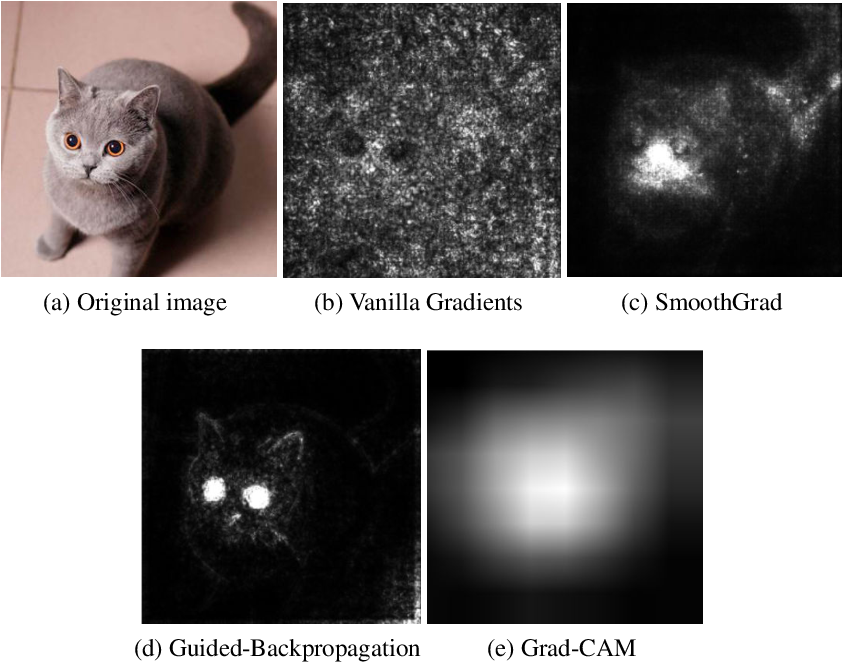
\includegraphics[width=\textwidth]{images/saliency_example.png}
    \caption{Explaining a black box prediction with saliency map.}
    \label{fig:saliencyExample}
\end{figure}

% Lấy ví dụ trong lĩnh vực y học, COVID-19 vừa qua đã là nguồn động lực to lớn để các nhà nghiên cứu giải quyết các vấn đề xung quanh nó nhằm chung tay góp sức đẩy lùi dịch bệnh. Đã có nhiều nghiên cứu sử dụng các mô hình học sâu để giải quyết các bài toán thị giác máy tính như nhận dạng điểm bất thường trên các ảnh chụp nội soi, XRay,.. Với sự phát triển của XAI, để chứng minh mô hình của mình đạt hiệu quả cao, các nhà nghiên cứu đã không còn chỉ quan tâm đến hiệu suất của mô hình bằng các phép đo (metrics) mà còn phải chứng minh được việc các mô hình có thật sự hoạt động như mong muốn bằng XAI bởi điều này không những ảnh hưởng đến tính minh bạch mà còn là niềm tin khi sử dụng trí tuệ nhân tạo để giải quyết vấn đề \cite{explainableCovidModel}.

% Tuy nhiên, XAI chính nó cũng tồn tại một vấn đề - Sự bất đồng giữa các phương pháp giải thích với nhau trên cùng một mô hình hộp đen (black-box model). Vấn đề này tuy quan trọng, nhưng lại chưa được nghiên cứu rộng rãi nói chung, đặc biệt là y học nói riêng. Nghiên cứu của Krishna và đồng nghiệp \cite{krishna_disagreement_problem} là một trong những nỗ lực đầu tiên nói lên vấn đề không đồng nhất này, bài báo đã chỉ ra sự không nhất quán giữa các mô hình XAI dựa trên tính quan trọng của đặc trưng trên các loại dữ liệu khác nhau như dữ liệu bảng, văn bản và hình ảnh. 

\section{Problems}
\label{sec:problem} 
There are numerous methods available for providing explanations for the outcome of a black box, but there is a challenge in assessing the quality of these explanations. Without a standard evaluation framework, there is a risk of using explanations that are baseless, ambiguous, or even contradictory. This is known as the disagreement problem and has recently been identified as a concern. Studies have investigated the severity of this problem for various types of explanation methods, but to the best of our knowledge, there seems to be a scarcity of studies specifically examining saliency maps.

The goal of XAI is to help users understand how complex AI systems work, thereby reducing incomprehensibility and increasing trust and confidence in the deployment of these systems. The disagreement problem poses a challenge to achieving this goal. If explanation methods do not agree on why the black box behaves in a certain way or provide conflicting explanations on what the black box considers important to its decision, it can cause confusion for users. Therefore, we believe this problem deserves the attention of XAI researchers and should be thoroughly studied.

% However, XAI itself faces a challenge - the disagreement between explanation methods for the same black-box model.  While this issue is important, it has not been extensively studied in general, particularly in the medical field. The research conducted by Krishna et al. \cite{krishna_disagreement_problem} is one of the first efforts to address this disagreement problem, demonstrating the inconsistency between XAI models based on feature importance across different types of data such as tabular, text, and image data.

\section{Objectives}
\label{sec:objective}
%Để đảm bảo độ tin cậy và hiệu quả của XAI trong lĩnh vực y tế, việc giải quyết vấn đề này là vô cùng quan trọng. Do đó, chúng tôi thực hiện nghiên cứu này nhằm đánh giá mức độ bất đồng giữa các phương pháp giải thích bằng cách tiến hành các thử nghiệm với nhiều phương pháp XAI khác nhau để giải thích một mô hình hộp đen trên tập dữ liệu về lĩnh vực y học.
While the disagreement problem has been recognized for various explanation methods, saliency maps have not been extensively studied in this regard, as mentioned in \ref{sec:problem}. Saliency methods are widely used to explain convolutional neural network (CNN) black boxes. With numerous techniques available and no consensus evaluation framework to guide their development, it is highly likely that some level of disagreement exists among these methods. Therefore, the purpose of this thesis is to investigate the disagreement problem among saliency methods. By doing so, we aim to shed light on various aspects of this problem and contribute to addressing it in the future.

% if we do not understand the reasons behind and address this issue, the results of deep learning models and their corresponding explanations will not be trustworthy, thereby potentially influencing many deep learning research outcomes. To tackle this issue, our study aims to thoroughly assess the extent of disagreement among explanation methods.

% Due to the limitations of time, our work does not directly provide a solution to this problem. Instead, our primary objective is to uncover the underlying causes of disagreement observed in different XAI methods when utilizing the saliency maps approach \cite{saliencyMaps} - focus on visualizing which parts of the input space attract attention and influence the model's output.

% There have been several previous studies raising concerns about the trustworthiness of saliency maps in the medical field \cite{trustworthiness} or whether such methods truly enhance the performance in explaining clinical outcomes \cite{assistGrading}. Their findings, however, suggest otherwise. By conducting experiments with various XAI methods to explain a black-box model on medical datasets by comparing saliency maps they produced, we believe that our research findings can contribute to identifying potential solutions for this issue.
\section{Methodology}
\label{sec:methodology}
%Để tìm ra lí do xảy ra những bất đồng, đầu tiên, chúng tôi phải chỉ ra những điểm bất đồng giữa các saliency maps được sinh ra. Để đánh giá mức độ bất đồng, chúng tôi dùng những độ đo ??? để so sánh phân bố các điểm nổi bật trên hai saliency maps với nhau.

In order to investigate the disagreement among saliency maps, we follow the current methodology utilized in existing literature. Initially, we train two distinct CNN models to serve as our designated target black boxes. Next, we opt for \numExperimentedMethods\ various saliency techniques and assess them over the aforementioned black boxes in order to obtain explanations. Subsequently, we measure the level of disagreement between the saliency methods for each black box by utilizing several metrics such as structural similarity index measure (SSIM) \cite{ssim}, feature agreement, sign agreement, and rank correlation.

Our analysis findings suggest that there is a substantial level of inconsistency among the explanation methods. We have also confirmed that this phenomenon persists across different types of black boxes, although there are intricate and diverse patterns of disagreement. We have concluded that the degree of disagreement is influenced not only by the type of explanation methods but also by the specific type of black box being explained. Additionally, we have noted a limitation in the sign agreement metric, which is approximately half of the feature agreement score. This may make it superfluous in measuring disagreement, and we therefore encourage researchers to develop advanced metrics that can capture a broader range of aspects of inconsistency.

Overall, the contributions of our thesis include:
\begin{itemize}
    \item Quantifying the degree of disagreement for \numExperimentedMethods\ saliency methods over two black boxes
    \item Highlighting the existence of disagreement for saliency maps methods
    \item Highlighting the variation of disagreement with respect to different kinds of black boxes
\end{itemize}

% To uncover the reasons behind these differencies, we first need to identify the points of difference among the generated saliency maps. To assess the level of difference, we employ measurement metrics including SSIM, feature agreement, sign agreement and rank correlation to compare the distribution of salient points between two saliency maps.
%Bằng cách so sánh từng cặp saliency maps trên tập dữ liệu test, ta có thể chỉ ra độ bất đồng giữa hai phương pháp giải thích khác nhau. Để thực nghiệm, chúng tôi sẽ chọn từ hai đến ba phương pháp theo từng loại phương pháp/thuật toán (phân loại theo hướng mà các phương pháp/thuật toán đó đang sử dụng để giải thích \cite{attributionbased}).
% By comparing each pair of saliency maps on the test dataset, we can determine the degree of difference between different explanation methods. 

%Độ bất đồng giữa các phương pháp với nhau trên từng độ đo sẽ được trực quan bằng bản đồ nhiệt. Từ đó, có thể rút trích được những hiểu biết (insights) như những huớng giải thích nào sẽ xuất hiện bất đồng với nhau, những độ đo nào làm nổi bật sự bất đồng hơn, ...
%Sau khi chỉ ra được điểm bất đồng, chúng tôi sẽ tìm lí do xảy ra vấn đề bằng cách phân tích sâu hơn về những yếu tố có thể gây bất đồng giữa các kết quả giải thích. Các yếu tố có thể kể đến như là: cách các thuật toán hoạt động, ý nghĩa của các saliency map được sinh ra bởi từng loại thuật toán. 


% \section{Contributions}
\label{sec:contributions}
In this research, we conducted experiments using saliency map-based explanation methods on a chest Xray dataset. The conclusions drawn from this study can potentially contribute to XAI in general, and specifically in the medical field. The following are the potential contributions:
\begin{itemize}
    \item Evaluating the accuracy of explanation methods in terms of localization utility.
    \item Identifying the disagreement trend among saliency map explanations.
    \item Identifying the reasons behind the discrepancies between different explanation methods, laying the foundation for further research to address this issue.
\end{itemize}
\section{Thesis Content}
\label{sec:thesisContent}
This thesis is organized into 6 chapters as followed:
\begin{itemize}
    \item In chapter \ref{ch:introduction} we introduce the context for our thesis and the problem that we focus on. We present the need for XAI in making complex models more interpretable to users and introduce saliency maps as a candidate solution. We then introduce the disagreement problem in which XAI methods differ from each other in explaining a complex black box. Finally, we state the goal of our thesis in attempting to study the disagreement between saliency methods, which currently lacks extensive research.
    \item In chapter \ref{ch:background} we provide an overview of XAI and some saliency-based methods. First, we cover XAI's history, growth, and classification of approaches in XAI. Then, we introduce two types of saliency-based explanation methods: gradient-based and perturbation-based and provide an overview of their general ideas.
    \item In chapter \ref{ch:relatedWorks} we discuss in detail the disagreement problem in XAI and introduce prior works that highlighted this problem. We also present several works on assessing the quality of saliency maps in practical use, since there is currently no work that highlights the disagreement between saliency-based methods specifically.
    \item In chapter \ref{ch:proposedMethod} we present our approach to quantifying the disagreement between saliency-based methods. First, we describe the mathematical formulation for four metrics we used to measure disagreement, including feature agreement, sign agreement, rank correlation (inherited and adapted for saliency maps from \cite{krishna_disagreement_problem}), and structural similarity index metric. Then, we select several methods (both gradient-based and perturbation-based) for generating explanations and two CNNs as black boxes (InceptionV3 and ResNet). We also provide an overview of the architecture of these two black boxes.
    \item In chapter \ref{ch:experimentsAndResult} we provide a detailed description of our experiment in measuring disagreement, as well as a discussion about our findings. First, we describe the dataset, the environment configurations we used, the two CNNs that we used as black boxes for our experiment, and how we measured disagreement. Then, we analyze the results and conclude some findings, which include a confirmation of disagreements among the explanation methods, a confirmation of complex disagreement patterns when evaluated on different black boxes, and an identified weakness in the established metric sign agreement in measuring disagreement.
    \item In chapter \ref{ch:conclusion} we conclude our thesis by providing a summary of our key findings, identifying some drawbacks in our work, and discussing future directions toward resolving the disagreement problem.
\end{itemize}